\chapter{Gestion de licences}
\label{ch:softs}


\section{Recherches initiales}
Lors de cette première partie de recherches, il a fallu réfléchir au problème des différentes étapes de l'ouverture et d'utilisation d'une application.
En effet, il a fallu découper les étapes à sécuriser et c'est pour cela que les recherches effectuées se sont axées autour de l'ouverture de l'application et des interactions de cette dernière avec le \gls{filesystem} de l'application.

\subsection{Ouverture d'une application}
Lors de l'analyse faite lors de cette première partie, il a fallu définir un use-case satisfaisant pour le comportement à adopter lors de l'ouverture d'une application.
En effet, il devait être déterminer quelle technologie sera utilisée pour containeriser une application.
La discussion s'axait autour de la virtualisation et l'émulation, deux procédés de simulation distincts.
Afin de bien définir chacun des termes, il est impératif de faire un détour pour ne pas se méprendre sur les termes employés : 

\begin{itemize}
	\item Simulation : "Représentation fictive de la réalité. Il s'agit d'imiter [et modéliser] une situation"\cite{sev}.
	\item Emulation : "Procédé permettant de reproduire à l'identique le comportement d’un logiciel et son architecture matérielle." \cite{sev} Il est donc possible de simuler une architecture différente de celle installée sur la machine.
	\item Virtualisation : Procédé de virtualisation utilisant les ressources physiques de l'ordinateur. Il n'est donc pas possible de simuler une architecture différentes de celle présente sur la machine.
\end{itemize}
 
Au terme de ces recherches, il a été possible d'établir une liste de points positifs et négatifs pour chacune de ces technologies.

Concernant l'émulation :
\begin{itemize}
	\item Avantages :
	\begin{itemize}
		\item Une machine entière peut être construite depuis un logiciel
		\item Les composantes hardware peuvent être construites de manière logiciel
		\item Possibilité d'émuler des architectures vétustes (PowerPC par exemple)
	\end{itemize}
	\item Inconvénients :
	\begin{itemize}
		\item Gourmand en ressources
		\item Exécution de code étranger au niveau du kernel et CPU en le convertissant en ASM
	\end{itemize}
\end{itemize}
Concernant la virtualisation :
\begin{itemize}
	\item Avantages :
	\begin{itemize}
		\item Meilleures performances car moins de compilation
		\item La virtualisation se fait directement sur le hardware natif
	\end{itemize}
	\item Inconvénients :
	\begin{itemize}
		\item Limitations au niveau du hardware car il est impossible de virtualiser une architecture qui n'est pas présente
	\end{itemize}
\end{itemize}
\cite{evs}
\cite{evs2}
\newline

% TODO : Faire des schémas pour l'émulation et virtualisation

Au fur et à mesure de l'avancement du travail, la virtualisation est ressortie comme le choix définitif de technologies de simulation.
Cela est dû au fait qu'il s'agit d'une technologie plus optimisée au niveau des ressources utilisées.
En effet, il faut impérativement que l'utilisation de ces applications soit la plus optimisée et fluide possible, et ce malgré la surcouche utilisée.
\newline
Suite à cela, il a fallu choisir une technologie, utilisant la virtualisation, permettant d'afficher l'interface graphique d'une application.
Quatres technologies sont ressorties, QEMU, Docker, Kubernetes et snap.
Docker permet de créer un environnement Linux complet, permettant donc d'installer et de gérer un \gls{filesystem} à part.
De plus, Docker permet de construire une image qui sera ensuite reproductible, ce qui permet d'avoir plusieurs instances de la même image en même temps.
Ce comportement est très avantageux dans la construction de notre architecture.
\newline
QEMU permet d'avoir des performances optimisées sur des petits systèmes ou de tailles moyennes.
Tous les aspects de la virtualisation sont optimisés. 
Cependant, au niveau de l'installation et la prise en main, cet outil est beaucoup plus complexe que les autres outils.
Le maintien d'un tel outil peut s'avérer plus complexe que certains autres outils. 
\newline
Kubernetes se veut être le nouveau Docker car les deux technologies utilise la containerisation afin de gérer une application.
Kubernetes permet d'abstraire certaines parties du procédé de containerisation, ce qui rend son utilisation plus légère.
Le soucis est que de par son abstraction, sa gestion avec le \gls{filesystem} peut être moins facile et malléable qu'avec Docker
Les deux technologies peuvent être utilisées ensemble sans soucis.
En effet, les outils peuvent être complémentaires et la combinaison des deux est très performante.
\newline
Snap permet de containeriser des application à travers un packet manager mais n'offre pas de \gls{filesystem} et ne permet pas de personnaliser le container à notre volonté.
De plus, selon beaucoup d'experts, snap ne doit en aucun cas être utilisé sur des systèmes comme Archlinux car il installe beaucoup de composantes inutiles.
Dans l'idée que le projet doit être portable, il faut qu'un utilisateur utilisant n'importe quel \gls{Operating System} puisse lancer une application containerisé.
\newline
Finalement, l'outil Docker a été choisi car c'est celui qui offre les performances les plus complètes et qui a un support et une communauté les plus fournis.
De plus, de part la maîtrise plus prononcée de Docker et sa maniabilité, il est apparu évident de choisir cet outil.
Docker permet d'avoir un \gls{filesystem} externe à celui natif et d'interagir avec ce dernier.


\subsection{Interactions avec le filesystem}

Après analyse des différents scénarios, il est apparu qu'il fallait aussi gérer les interactions avec le \gls{filesystem} entre le container et le natif.
L'idée recherchée était de mettre en place un système permettant d'écrire sur le système natif seulement si le fichier modifié est authentifié comme travail de l'école.
Dans ce but, il est nécessaire de créer un système de signatures de fichiers qui émet un signal au \gls{filesystem} que le container peut écrire.
Cela implique que les professeurs devront mettre en place un système de distribution de fichiers qui seront authentifiés au préalable.
L'idée serait de mettre en place une autorité de vérification qui peut signer les fichiers envoyés sur le serveur.
Avec ce système, le container Docker ne pourrait écrire sur le \gls{filesystem} natif si et seulement si la signature est valable.
Si la signature est valable, un signal sera envoyé au Docker et lui permettra d'écrire de manière persistante les données de l'utilisateur.
Pour ce faire, il est possible d'implémenter un script Python qui gère l'envoi et la réception des signaux système et qui communique avec le \gls{filesystem} du container Docker.
\newline
Lors d'un point de situation hebdomadaire, M. Kapfer a mis en avant des soucis de sécurité avec l'approche prise jusqu'à maintenant.
En effet, l'utilisation de Python dans la gestion des interactions avec le \gls{filesystem} peut poser des problèmes de modifications du script.
En effet, Python n'étant pas un langage compilé, il est possible de retrouver le code source du script et donc de le modifier.
De plus, il évoque la complexité de créer une autorité de signatures et le problème de vérification du fichier signé.
\newline
Une solution aurait été de mettre les scripts d'installation dans un dossier appartenant à un utilisateur système, dont personne n'a le mot de passe, et qui n'a aucun droit sur le système à part l'exécution de ces scripts.
Cela aurait complexifié les interactions au niveau du \gls{filesystem} et du container Docker.
De plus, aucune solution n'a permis de simplifier la création de l'autorité de certification.
\newline
Une autre solution, suggérée par M. Kapfer, serait d'utiliser une infrastructure client-serveur qui communique à travers une technologie \acrshort{vnc}.
Le serveur aurait une partie disque propre à chaque étudiant ou professeur.
Les applications ne seraient pas installées sur l'ordinateur de l'étudiant mais sur le serveur et accessible via un client Web.
\newline
Au terme de plusieurs discussions et réflexions, il apparaît clairement que cette dernière approche est celle à choisir.
Le système de lancement d'application resterait le même, mais serait déporté sur un serveur distant.
\newline
Avec l'adoption de cette approche, il est impératif de savoir si l'utilisation de la technologie \acrshort{vnc} sur un client Web.
En regardant sur différents types d'articles, il est ressorti qu'il était possible de faire une telle action en utilisant un serveur CentOs.\cite{vnc}
L'utilisation d'une telle distribution Linux permet de pouvoir gérer plus facilement certains aspects de droits utilisateurs sur un fichier.
En effet, la configuration des \acrfull{acl} et des permissions classiques permet de pouvoir gérer les droits de modification, de lecture. d'ajout, de suppression et bien d'autres sur un fichier ou un dossier.
De ce fait, il est possible d'envisager que sur le serveur, un utilisateur puisse effectuer une action et un autre ne le puisse pas.
Cela permettra de mettre en place des rôles distincts pour les professeurs et pour les étudiants.
\newline
Il est possible de rajouter une couche de sécurité pour gérer les aspects de containerisation du tunnel \acrshort{vnc}.
Un servlet du nom de \textit{Guacamole} permet de diffuser une fenêtre \acrshort{vnc} pour un utilisateur donné avec une paire "username:password".

\section{Spécifications}

\subsection{Configuration du serveur}
Lors de la configuration du serveur, il faut installer une version de CentOs 7.
Une autre version ne permet pas l'installation "simple" de certaines composantes essentielles telle que \textit{php5.5}, \textit{guacamole} pour ne citer qu'elles.
Il est nécessaire d'avoir une interface graphique pour faire marcher le \acrshort{vnc} de manière correcte.
Une fois le serveur installé, il faut configurer les différents composantes permettant de mettre en place le \acrshort{vnc}.
Il faut donc installer le \acrshort{vnc} Server \cite{vncs} permettant d'indiquer au client qu'il faut regarder à un endroit donné du \gls{filesystem}.
Sur ce serveur, il faut distinguer trois rôles distincts :
\begin{itemize}
	\item Admin
	\item Teacher
	\item Student
\end{itemize}
En effet, chaque rôle pourra faire des actions différentes.

\begin{figure}[H]
	\centering
	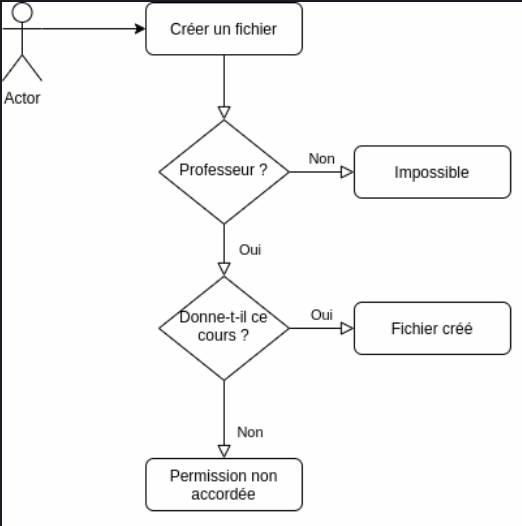
\includegraphics[scale=0.45]{images/create.png}
	\caption{Création de fichiers}
	\label{fig:create}
\end{figure}


\begin{figure}[H]
	\centering
	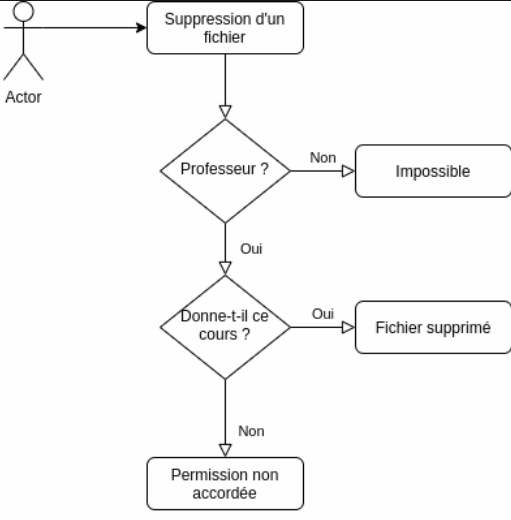
\includegraphics[scale=0.45]{images/delete.png}
	\caption{Suppression de fichiers}
	\label{fig:delete}
\end{figure}


\begin{figure}[H]
	\centering
	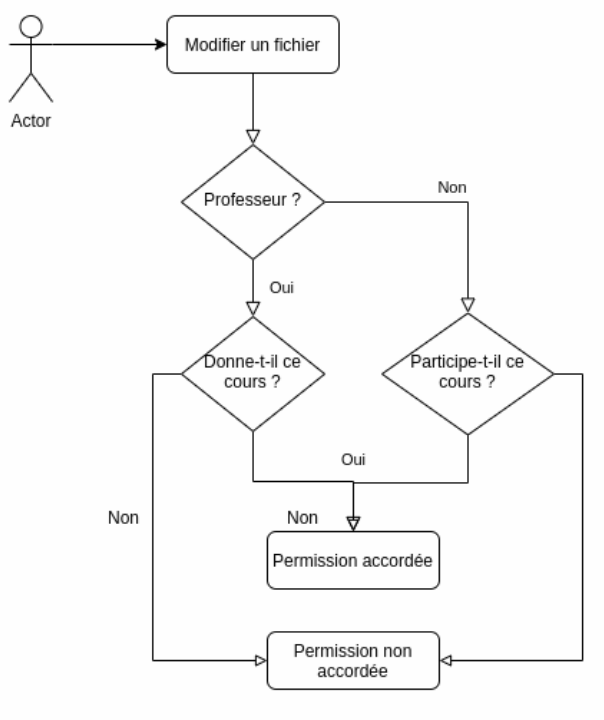
\includegraphics[scale=0.45]{images/edit.png}
	\caption{Modification de fichiers}
	\label{fig:edit}
\end{figure}


\begin{figure}[H]
	\centering
	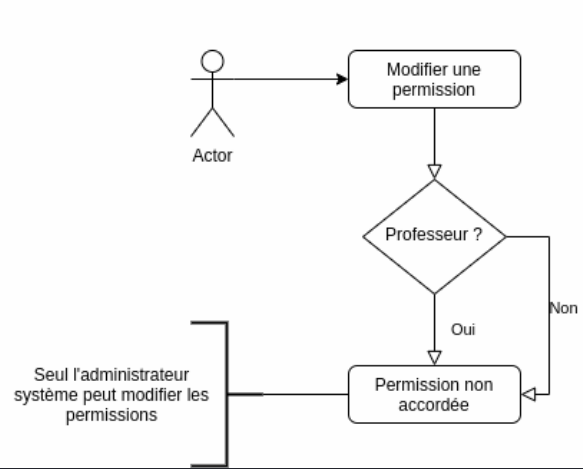
\includegraphics[scale=0.45]{images/perms.png}
	\caption{Modification des permissions}
	\label{fig:perms}
\end{figure}

L'administrateur peut évidemment modifier, rajouter et supprimer des fichiers.
\newline
Toute ces cas peuvent s'appliquer grâce à l'utilisation d'une base de données, en \textit{PostgresQL} par exemple.
% TODO : Vérifie le graph SQL pour ne rien oublier !
La base de données est très simple et comprend quatre tables comme présenté ci-dessous :
\begin{figure}[H]
	\centering
	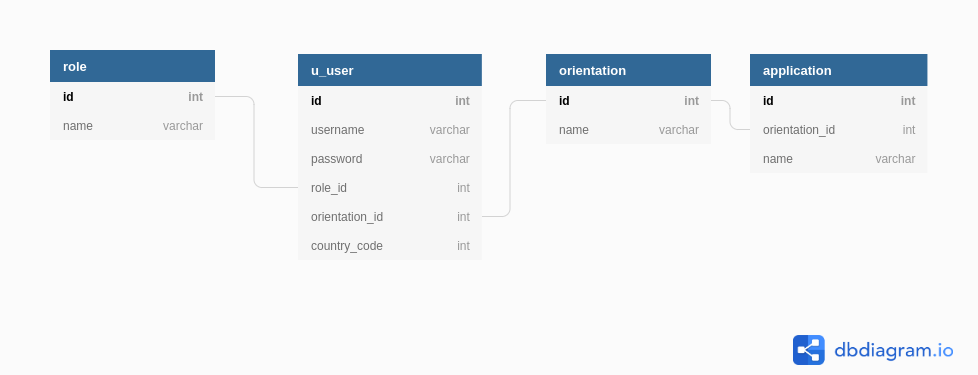
\includegraphics[scale=0.45]{images/DB.png}
	\caption{Base de données}
	\label{fig:db}
\end{figure}
L'utilisation de cette base de données permet de créer un espace utilisateur pour chacun des étudiants ou professeurs présents dans la table \textit{u\_user}.
En fonction de l'orientation d'un utilisateur, une liste d'applications lui est attribuée.
Un dossier est créé pour chaque application avec un script bash de lancement à l'intérieur.
Lors de la création d'une connexion sur le client Web, ce dernier appellera le script correspondant à l'application souhaitée.


\subsection{Client Web}
Le client Web a pour but de donner une fenêtre de lecture aux étudiants, leur permettant de choisir les applications à lancer depuis leur navigateur.
L'accès à ce site sera protégée et accessible avec les identifiants AAI. 
De ce fait, il est possible d'utiliser la technologie php pour aller faire les vérifications sur la base de données créée au préalable.
Ensuite, une liste d'applications, propre à chaque étudiant, sera dressée et avec une simple sélection de l'application.
Une interface utilisateur permet de voir le nombre d'applications disponibles pour chaque étudiant, de voir l'espace disque disponible sur le serveur et une liste de devoirs mise à disposition par les professeurs.
Tout le code mis en place dans cette partie sera fait en \textit{HTML5}, \textit{CSS3}, \textit{PHP} et \textit{Javascript}.
Le flot général sur le site est le suivant :
\begin{figure}[H]
	\centering
	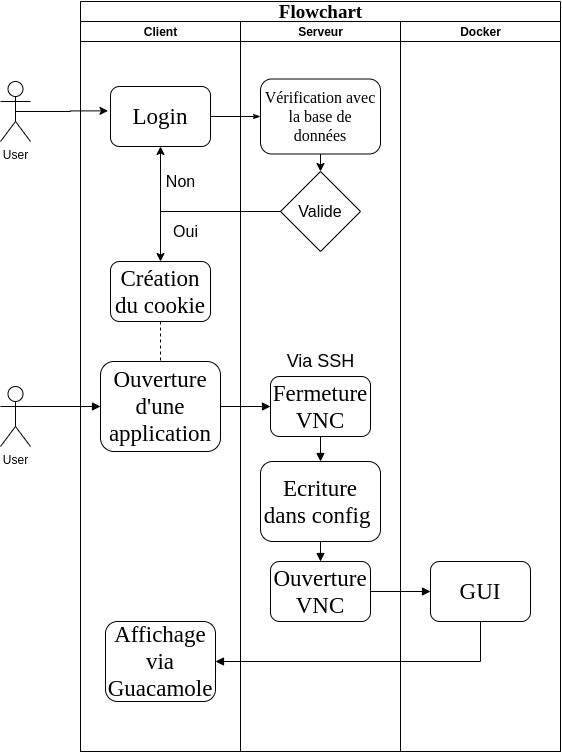
\includegraphics[scale=0.35]{images/client_flow.png}
	\caption{Flot des actions sur le site lors de l'ouverture d'une session et d'une application}
	\label{fig:client_flow}
\end{figure}

\subsection{Ouverture de l'application}
Lors de la phase d'ouverture, après la sélection de l'utilisateur dans son navigateur, tout se passe du côté du serveur.
La sélection utilisateur permet de déclencher un appel à un script bash qui lancera l'application containerisée avec Docker.
L'image du container sera construite au préalable mais le script vérifiera quand même si tel est bien le cas.
Ensuite, il faut configurer le \acrshort{vnc} pour qu'il ne diffuse que la fenêtre entrain de se lancer et pas de fenêtres de Terminal ou de gestionnaire de fichiers.
Lors de l'appel par le client Web, le serveur \acrshort{vnc} exécuté sur le serveur pour un étudiant est arrêté, le fichier de configuration modifié de sorte à lancer la bonne application et relancé pour enfin diffuser l'application sur le client.

\begin{figure}[H]
	\centering
	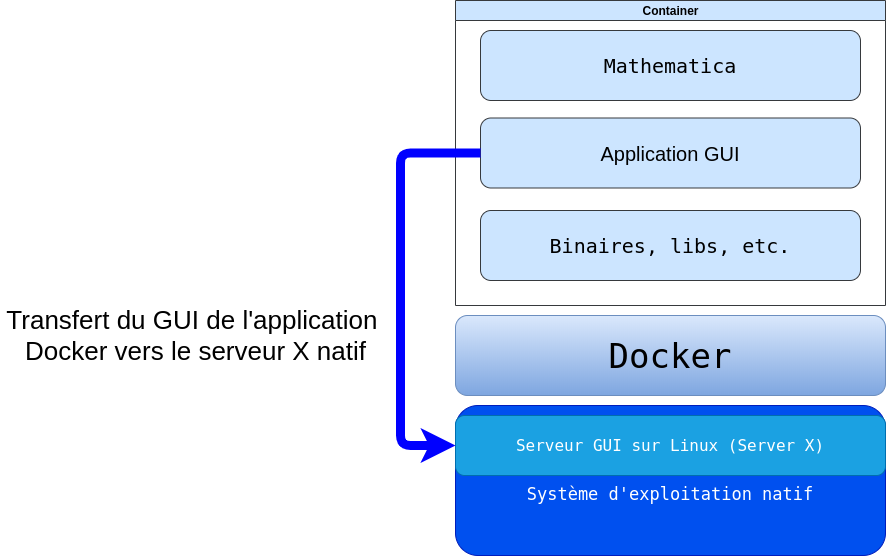
\includegraphics[scale=0.35]{images/container.png}
	\caption{Container Docker avec application GUI}
	\label{fig:cont}
\end{figure}


%TODO : Faire un schéma du script !
\subsection{Containerisation des application}
Afin de containeriser une application, il est nécessaire de créer un Dockerfile définissant les règles de construction de cette dernière.
Il est, à priori, impossible d'automatiser ce processus car chaque application demande des pré-requis spécifiques.
En revanche, une base commune permet de comprendre et de rendre l'écriture de ces fichiers de configurations et de rendre le lancement plus simple.
En effet, les applications arrivent à se lancer en mode GUI grâce à un partage de ressources avec l'aide d'un volume.
Il faut mettre en commun la ressource graphique de la machine hôte et passer en variable d'environnement le numéro de "display", par défaut \textit{:0}.
De ce fait, il est possible d'établir un \textit{template} avec les lignes directrices du Dockerfile mais pas de généraliser sa construction.
De par la configuration du serveur, il est impossible pour le Docker de traverser les dossiers, ce qui rend l'écriture dans une autre partie impossible.
De plus, Docker ne peut pas créer ou supprimer des fichiers, seulement modifier un fichier existant, grâce à la configuration du serveur.
Chaque application aura un container séparé, ce qui limite les risques d'intrusion et d'interactions non-contrôlées.
Les containers ne seront pas atteignables depuis l'extérieur du réseau du serveur.
Cela permettra de limiter encore une fois la surface d'attaque depuis l'extérieure.

\subsection{Interactions avec le filesystem}
Les interactions entre le \gls{filesystem} du container et le \gls{filesystem} natif doivent être régulées selon les figures \ref{fig:create} \ref{fig:delete} \ref{fig:edit} \ref{fig:perms}.
Cela peut être grâce aux configurations des ACLs sur le serveur.
Ce procédé suffirait à garantir qu'aucun étudiant ne pourrait utiliser les logiciels fournis par l'école de manière illicite.
Les professeurs fournissent le fichier sur l'espace personnel des étudiants et les étudiants ne peuvent que modifier le fichier en question.
Il n'est alors plus nécessaire d'avoir une gestion des actions à l'intérieur même du container Docker.
De même façon qu'un utilisateur ne pourra pas rajouter de fichiers sur son \gls{filesystem}, Docker ne pourra pas le faire non plus.
Docker doit pouvoir prendre les fichiers présents dans le dossier et doit pouvoir écrire seulement si le fichier existe au préalable.
Cela est réalisable lors du \textit{run} du container Docker. 
Le fait de partager un volume entre le \gls{filesystem} natif et celui du Docker permet de garantir qu'il n'y aie pas de modifications à un autre endroit que sur le dossier partagé.

\section{Architecture}
\begin{landscape}
	\begin{figure}[H]
		\centering
		\includegraphics[scale=0.55]{images/VNC&server_1.png}
		\caption{Architecture et comportement}
		\label{fig:arch1}
	\end{figure}
	\begin{figure}[H]
		\centering
		\includegraphics[scale=0.55]{images/VNC&server_2.png}
		\caption{Architecture et comportement}
		\label{fig:arch2}
	\end{figure}
	\begin{figure}[H]
		\centering
		\includegraphics[scale=0.55]{images/VNC&server_3.png}
		\caption{Architecture et comportement}
		\label{fig:arch3}
	\end{figure}
		
\end{landscape}

\section{Implémentation}

\subsection{Docker}

Afin de créer un container avec GUI, il est nécessaire de transférer l'environnement graphique du container vers celui de l'ordinateur hôte. 
Cela consiste à signaler au Docker qu'il doit utiliser une ressource partagée via le Dockerfile. 
Dans le Dockerfile ci-dessous, il est possible de voir qu'une variable d'environnement \com{ENV DISPLAY :0} est passée au container.
Cette variable permet de signaler le composant graphique à utiliser par le container.
\newline
Ensuite, il faut savoir quelles sont les dépendances du programme à installer et donc les passer en commande de construction du container.
Afin de minimiser la taille de l'image, il faut concaténer autant que possible les commandes ensemble. 
En reprenant le Dockerfile ci-dessous, il est possible de dégager certaines parties essentielles du fichier.
\newline
La première ligne sert à définir la version d'Ubuntu à utiliser.
Dans le cas actuel, il est recommandé d'utiliser Ubuntu 18.04.
Ensuite, il est nécessaire de copier tous les fichiers d'installation vers le container.
Il est possible de les placer dans un dossier arbitraire, mais recommandé de les mettre dans \com{/data}.
\newline
Les commandes des lignes 7 et 8 servent à définir la zone géographique du container.
Cette étape n'est pas nécessaire dans la majorité des cas mais dans le cas de Mathematica, il est obligatoire de le faire.
Ensuite, il est obligatoire d'installer les mises à jour et la commande  \com{sudo}.
Efin, il est recommandé de créer un utilisateur lambda, \textit{user} dans le cas actuel, afin de ne pas donner tous les droits à l'utilisateur final.
Après avoir créé cet utilisateur, il faut finalement installer toutes les dépendances de l'application. 
C'est à cause de cette partie qu'il est impossible de rendre la création des Dockerfile générique.

\inputsourcecode{bash}{"source_code/Dockerfile"}{Dockerfile}

Une fois le Dockerfile écrit, il est possible de lancer un script permettant de lancer le container.
Ce script permet de regarder dans le \gls{filesystem} natif si l'image a déjà été construite.
Si l'image est déjà construite, le script ne fait qu'appeler \com{docker run}.
Dans le cas où l'image n'est pas construite, il est impossible de construire l'image depuis un espace étudiant.
Seuls les professeurs ou les administrateurs pourront avoir accès au Dockerfile.

\inputsourcecode{bash}{"source_code/launch.sh"}{launch.sh}

L'appel à \com{docker images -q john:doe} permet de savoir si l'image existe ou non.
\begin{listingsbox}{console}{Docker images}
user@user:~$ docker images -q fsmdbfsdnfdssdhfsd:asashdalk
user@user:~$
\end{listingsbox}
La sortie de l'appel à cette fonction sera vide si l'image n'existe pas.
\newline
Si l'image existe, l'identifiant sera en sortie :


\begin{listingsbox}{console}{Docker images}
user@user:~$ docker images -q test:latest
7d7d5f60428a
user@user:~$
\end{listingsbox}

Lors de l'appel à \com{docker run}, il faut préciser où se trouve l'instance de Server X sur l'ordinateur hôte et de créer un volume partagé entre le container et l'hôte.
\newline
Les exemples utilisés pour ce travail sont Mathematica, comme montré ci-dessus, et Logisim qui se trouvera en annexe.
La raison pour laquelle il a été choisi de prendre ces logiciels comme exemple est que l'un est un logiciel demandant beaucoup de ressources matérielles pour certains calculs et l'autre est utilisé de manière concrète lors de certains cours donnés par le \textit{REDS}.


\subsection{Configuration du serveur}

Afin de configurer le serveur, le service informatique de l'école avait été contacté. 
Il aurait été souhaitable d'avoir une machine virtuelle sur les serveurs de développement de l'école afin de pouvoir travailler en conditions de production.
Malheureusement, la configuration graphique du serveur n'a pas pu être possible et malgré la communication avec le responsable, une solution n'a pas pu être trouvée.
\newline
De ce fait, afin de simuler au plus proche possible le serveur, tout le travail a été fait sur machine virtuelle.
Après l'installation de CentOs 7, il a fallu créer une base de données en PostgresQL.
A l'aide de la requête ci-dessous, il est possible de récupérer les informations suivantes : 
\begin{itemize}
	\item Username
	\item Password
	\item Rôle
	\item Applications
	\item id
\end{itemize}

\begin{listingsbox}{SQL}{Requête}
SELECT u.username, u.password, r.role_name, 
array_to_string(array_agg(a.name), ',') AS Applications, u.user_id 
FROM u_user u INNER JOIN role r ON u.role_id = r.role_id 
INNER JOIN orientation o ON u.orientation_id = o.orientation_id 
INNER JOIN application a ON a.orientation_id = o.orientation_id 
GROUP BY u.user_id, u.username, u.password, r.role_name;
\end{listingsbox}

La spécificité de cette requête est cette partie : \com{array\_to\_string(array\_agg(a.name), ',')}. 
La première partie crée un tableau depuis la valeur des noms d'applications qui sont en commun avec la cause \textit{GROUP BY} de la fin de requête.
Une fois ce tableau créé, il est transformé en chaîne de caractères pour qu'il soit lisible dans les scripts suivants : 

\inputsourcecode{bash}{"source_code/.env"}{.env}
\inputsourcecode{bash}{"source_code/update_csv"}{update\_csv}
Les options utilisées pour appeler la base de données et l'exporter en \textit{.csv} sont les suivantes : 
\begin{itemize}
	\item \com{-t} : Supprime les noms de colonnes
	\item \com{-A} : Supprime l'alignement
	\item \com{-h} : Le nom de l'hôte de la base de données
	\item \com{-p} : Numéro de port
	\item \com{-d} : Nom de la base de données
	\item \com{-U} : Nom d'utilisateur de la base de données
	\item \com{-c} : Commande à exécuter
\end{itemize}

Avec le script situé dans le même dossier, \com{create\_user}, il est possible de lire le \textit{.csv} créé et d'ajouter un nouvel utilisateur si le fichier a été modifié.

\inputsourcecode{bash}{"source_code/create_user"}{create\_user}

Les deux scripts sont appelé dans le script \com{main} qui doit être appelé avec un utilisateur avec les droits \com{sudo}.
Une façon d'enlever les demandes de mots de passe et d'ajout de la commande \com{sudo} est d'ajouter l'exécution de la commande \com{main} dans les \textit{sudoers} et d'ajouter un alias pour enlever le \com{sudo}.

\inputsourcecode{bash}{"source_code/main"}{main}

\begin{listingsbox}{bash}{sudoers \& alias}
# Dans les sudoers
jeremy ALL=(root) NOPASSWD: /home/jeremy/docker/main
# Dans la configuration du terminal (bash, zsh, etc.)
alias main='sudo /home/jeremy/docker/main'
\end{listingsbox}
Bien évidemment, il faudra remplacer le chemin d'accès au script avec le bon chemin.


\subsection{Configuration de guacamole}

Afin de configurer le servlet Guacamole, il a fallu suivre le tutoriel de Deviant Engineer \cite{guac}.
Après la configuration initiale, il a fallu créer un alias et ajouter \com{guacd} aux sudoers car il était impossible de lancer le servlet sans cette manipulation.
\begin{listingsbox}{bash}{sudoers \& alias}
# Dans les sudoers
jeremy ALL=(root) NOPASSWD: /usr/local/sbin/guacd -f
# Dans la configuration du terminal (bash, zsh, etc.)
alias guacd='sudo /usr/local/sbin/guacd -f &'
\end{listingsbox}
Une fois le daemon lancé, il a fallu configurer le serveur \acrshort{vnc}.
Pour ce faire, il est nécessaire d'installer \textit{Tiger VNC}.
Sur CentOs, il a suffi de suivre le tutoriel proposé par Pradeep Kumar \cite{vnc_conf}.
Ensuite, comme montré dans le scripte "\textit{create\_user} ci-dessus, il est obligatoire de configurer correctement les fichiers d'utilisateurs de guacamole, situé dans \com{/etc/guacamole/user-mapping.xml}.
\begin{listingsbox}{xml}{Exemple d'utilisateur dans user-mapping.xml}
<authorize username="jeremy" password="pass">
	<protocol>vnc</protocol>
	<param name="hostname">localhost</param>
	<param name="port">5901</param>
	<param name="password">polopolo</param>
</authorize>
\end{listingsbox}
Le nom d'utilisateur et le mot de passe sont donnés de manière arbitraire et permettent d'identifier un utilisateur sur le client.
Le protocole doit être spécifié car il est possible de faire du \textit{RDP}, du \textit{SSH}, \textit{VNC} ou du \textit{Telnet}.
Le nom de l'hôte correspond à l'adresse sur laquelle le serveur \acrshort{vnc} a été configuré.
Le numéro de port doit être le même que celui ouvert par le serveur \acrshort{vnc}.
Enfin, le mot de passe est celui défini lors de la configuration du serveur \acrshort{vnc}.
\newline
De manière à rendre le serveur Guacamole opérationnel, il est nécessaire de faire un appel à l'alias créé au préalable.
\begin{figure}[H]
	\centering
	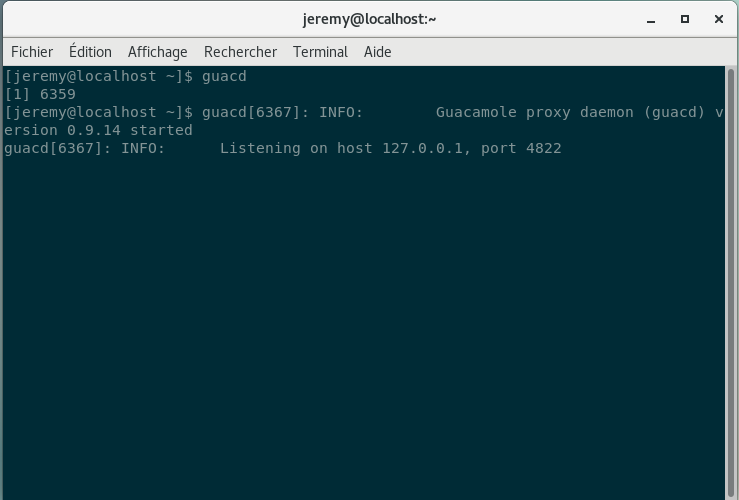
\includegraphics[scale=0.55]{images/guacd.png}
	\caption{Appel à \com{guacd}}
	\label{fig:guacd}
\end{figure}

Le client est accessible à l'adresse suivante : \com{localhost:8080/guacamole}.
\begin{figure}[H]
	\centering
	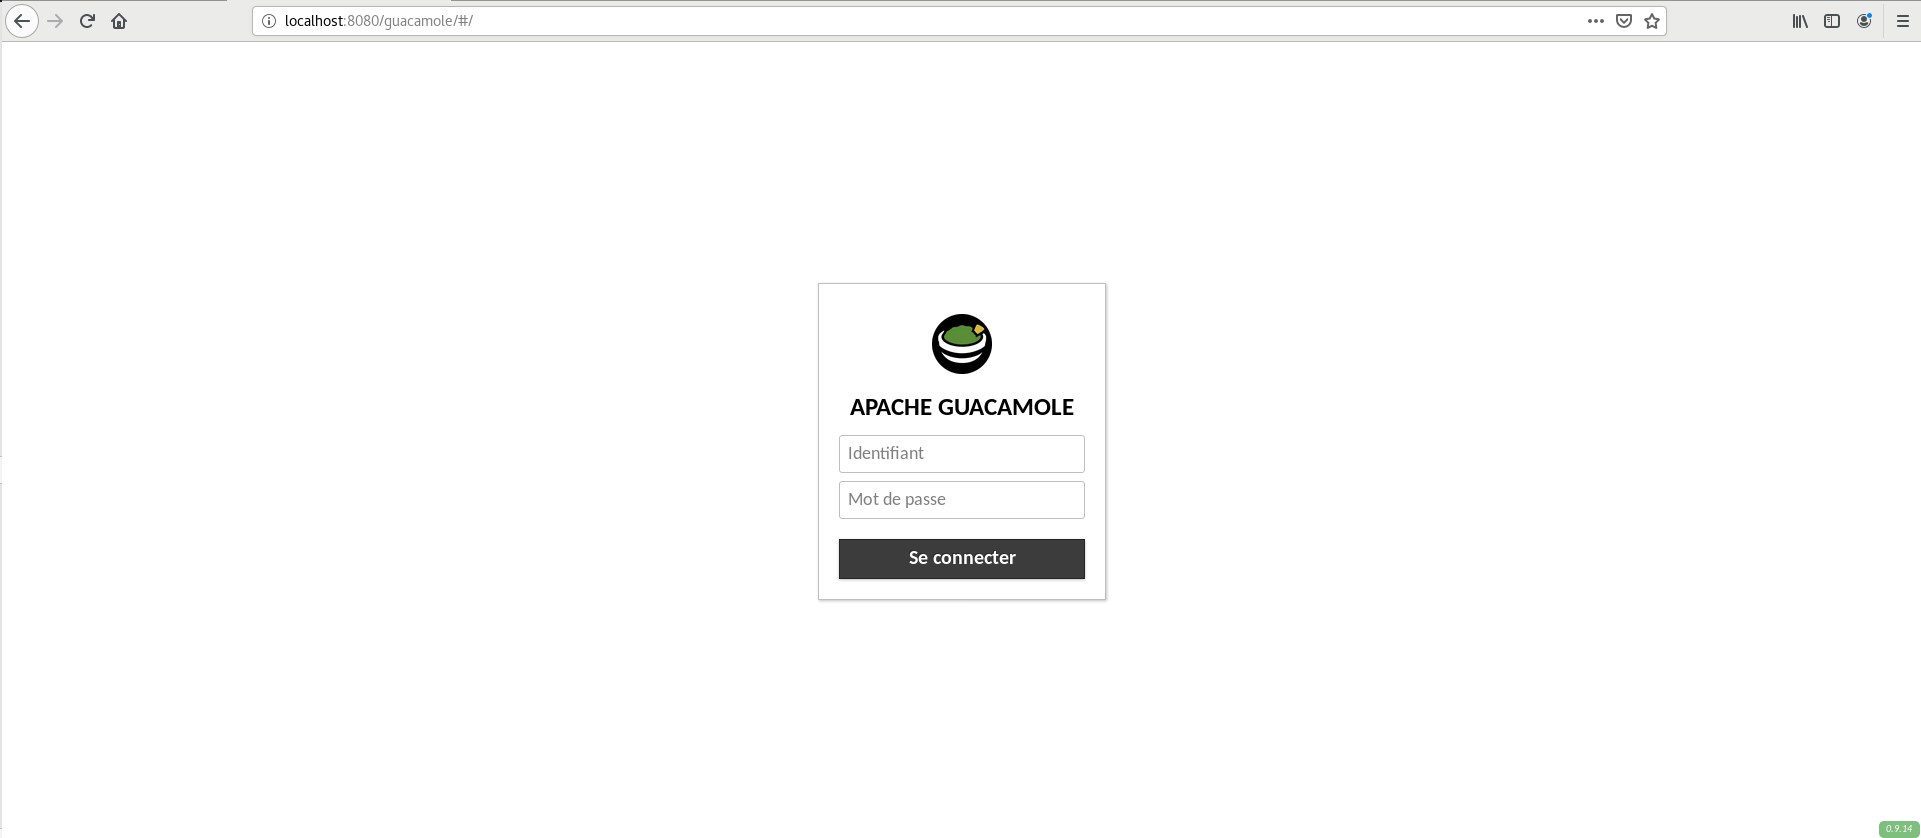
\includegraphics[scale=0.2]{images/guacd_client.png}
	\caption{Page d'accueil de Guacamole}
	\label{fig:guacd_client}
\end{figure}

\subsection{Site internet}
Pour commencer le développement du site, un template libre de droit a été trouvé sur le site de Creative Tim \cite{creatim}.
Une fois le site copié, il était possible de personnaliser l'interface utilisateur au bon vouloir du projet.
Il a fallu rajouter un accès à la base données et pour ce faire, la base de données créée lors de la configuration du serveur a été réutilisée.
\newline
En utilisant la technologie \textit{php-pqsql}, il est possible de faire des requêtes sur une base de données en Postgres avec l'aide de PHP.
Par exemple, pour établir une connexion, il suffit de faire : 
\inputsourcecode{bash}{"source_code/conn_db.php"}{Connexion à la base de données via PHP}
\begin{figure}[H]
	\centering
	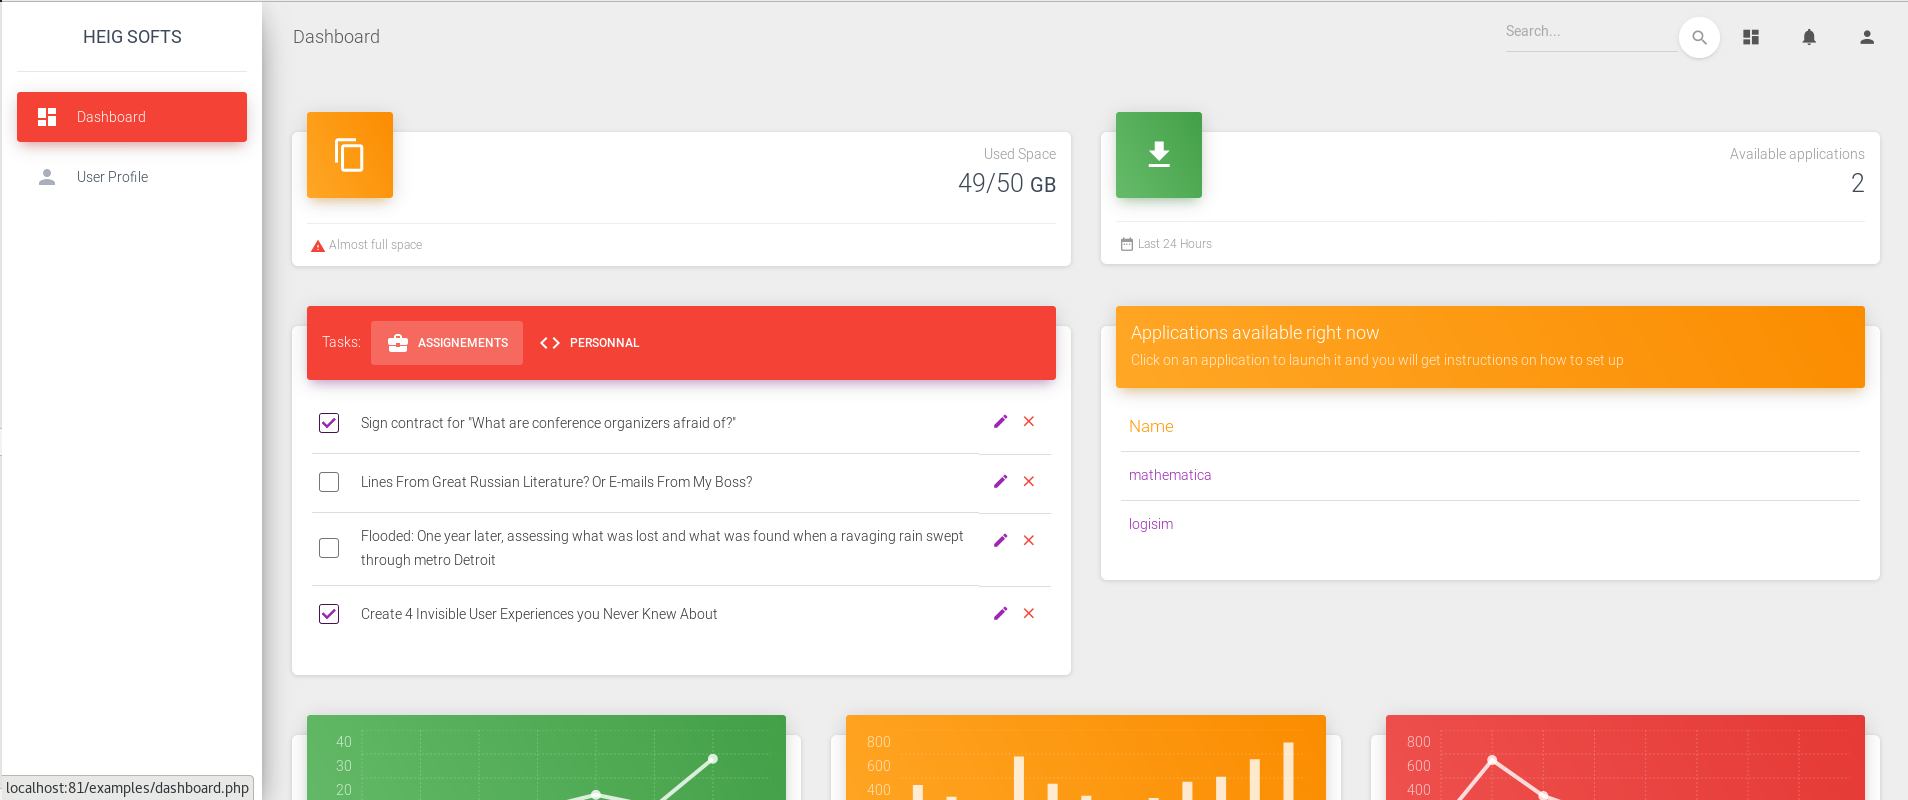
\includegraphics[scale=0.2]{images/website.png}
	\caption{Page d'accueil du site}
	\label{fig:website}
\end{figure}
Le site prend l'aspect d'un tableau de bord. 
Sur la droite apparaissent les applications disponibles. 
En cliquant sur l'une d'elles, il est possible d'accéder à la page d'affichage de l'application.
Sur la gauche se trouve une liste de devoirs mis à disposition par le professeur.
Pour le moment, cette fonctionnalité n'est pas disponible mais l'exemple est présent pour montrer comment le rendu final serait.
Pour implémenter cette fonctionnalité, il faudra rajouter plusieurs tables dans la base de données :
\begin{itemize}
	\item \textbf{Spécifications de "teacher" et "student"} : Deux tables qui héritent de \textit{u\_user} et qui permettent à un professeur de distribuer des devoirs aux étudiants qui suivent son cours.
	\item \textbf{homework} : Chaque devoir aura un numéro d'identification spécifique, une description et une date de rendu.
	\item \textbf{class} : Chaque classe aura un numéro d'identification spécifique, un nom et un professeur.
	\item \textbf{follows\_class} : Table de liaison permettant de dire si un étudiant suit une classe ou non. Elle contient l'id d'une classe et l'id d'un étudiant.
\end{itemize}

Une fois que l'utilisateur a fait une sélection d'application, le site redirige vers la page d'application.
Dans l'exemple ci-dessous, l'utilisateur a cliqué sur Logisim : 
\begin{figure}[H]
	\centering
	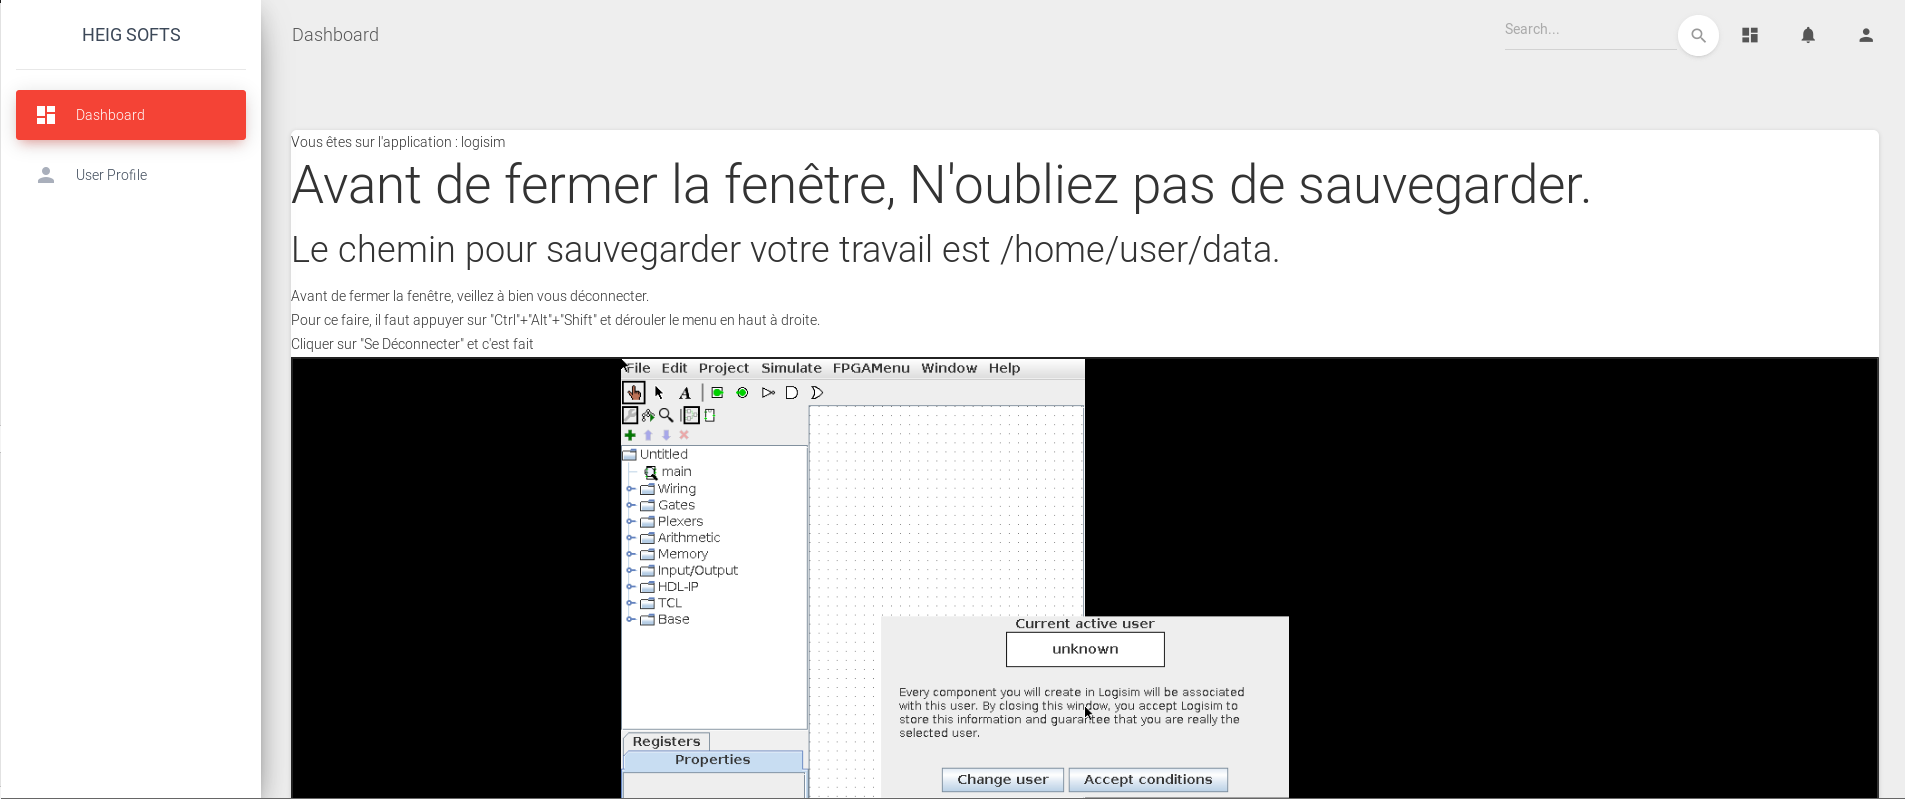
\includegraphics[scale=0.2]{images/website_logisim.png}
	\caption{Logisim}
	\label{fig:website_logisim}
\end{figure}
L'utilisateur peut donc modifier les fichiers présents dans le dossier partagé ou en rajouter s'il est administrateur.
La sauvegarde se fait dans tous les containers dans le dossier \com{/home/user/data}.
\newline
Pour avoir la fenêtre Guacamole sur l'interface, il est nécessaire de faire tourner deux services Web en parallèle.
Il faut configurer Tomcat de manière normale et avoir le client Guacamole sur le port 8080 du serveur.
En revanche, étant donné que ce travail a dû être fait sur une machine virtuelle,
afin de pouvoir avoir un rendu avec du \textit{PHP}, il faut faire tourner \textit{httpd} sur le port 81 et non 80 ou 8080.
Ensuite, à l'aide d'une iframe, il est possible d'appeler la page du client Guacamole avec dans l'url la paire "username:password" pour avoir un login automatique.
\newline
L'espace utilisateur sert simplement à montrer les informations de l'utilisateur connecté.
Il est envisageable d'ajouter une option pour les professeurs et administrateurs d'ajouter une application à un étudiant ou d'enlever à un étudiant, l'accès à une application.
Pour le moment, ce n'est pas encore implémenté.

\section{Tests}

\subsection{Serveur}
Les tests sur le serveur ont majoritairement porté sur la création des utilisateurs et le lancement du serveur \acrshort{vnc} avec les bons ports ouverts et le fichier de configuration guacamole écrit correctement.
Il a fallu tout d'abord lancé le script \com{main} et attendre la fin de son exécution. 
Le comportement attendu à la fin, avec la base de données actuelles, est : "trois utilisateurs avec leurs dossiers \com{/home} respectifs ont été créés".
Il faut aussi prendre en compte la population de ce dossier avec les répertoires contenant les fichiers de lancement des applications : \com{/home/<user>/<application>/launch.sh}.
\newline
Le script \com{main} finit son exécution sans encombre.
Une fois terminé, il est possible de voir les dossiers utilisateurs créés.
\begin{figure}[H]
	\centering
	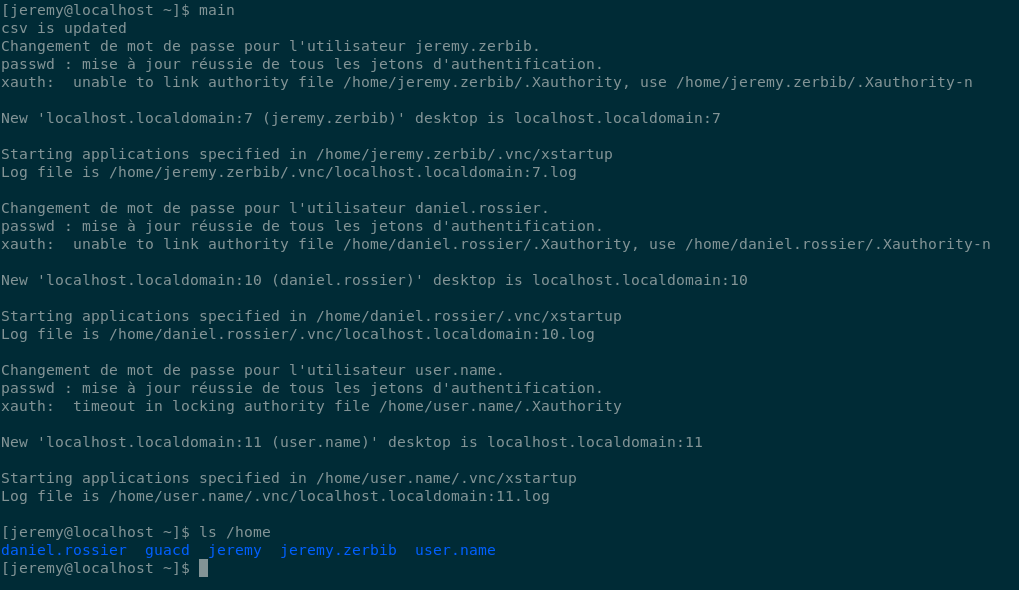
\includegraphics[scale=0.2]{images/main_home.png}
	\caption{Création des dossiers utilisateur}
	\label{fig:main_home}
\end{figure}



\subsection{Docker}

Une première phase de tests a été faite sur une machine utilisateur.
Cette phase consistait à tester le cloisonnement des applications avec l'ordinateur local.
Un volume partagé entre l'espace de \textit{test} et le container est créé permettant de rendre certains fichiers de configuration persistant et les travaux d'être sauvegardés.
Ce procédé est possible grâce à l'option suivante lors de l'appel à \com{docker run} : "\com{-v \${HOME}/logisim/data:/home/user/data}"
\newline 
Les tests ont donc consisté à lancer le container Mathematica et créer un nouveau fichier.
Il est possible de sauvegarder sur le filesystem du container le fichier créé mais il est impossible de le sauvegarder sur le filesystem de \textit{test}.
Après fermeture du container, aucun nouveau fichier n'est présent sur le \gls{filesystem} de \textit{test}.
Ce que cela implique est que si le fichier est sauvegardé  n'importe où à part le volume partagé, il est possible d'écrire en mémoire.
\newline 
Ensuite, un fichier est créé sur le volume partagé entre \textit{test} et le container en préambule de l'ouverture de ce dernier.
L'utilisateur a la possibilité de modifier le fichier et lors de la fermeture du container, il est possible de voir que le fichier modifié est présent dans le dossier.
\newline
Ensuite, il fallait vérifier que depuis le serveur, l'utilisateur puisse écrire sur un fichier donné et que suivant son rôle, il puisse ou non en créer un nouveau.
Dans tous les cas, il était impossible de créer un fichier depuis la plateforme Web.

\subsection{Guacamole}
Deux batteries de tests ont été faites sur Guacamole.
La première sur la page du client directement et la deuxième sur le site Internet afin de tester les interactions entre le servlet et la plateforme utilisateur.
\subsubsection{Client Guacamole}
Lors de l'arrivée sur la page du client Guacamole à l'adresse \com{localhost:8080/guacamole}, il est demandé de remplir un formulaire avec les identifiants d'un utilisateur.
Ces identifiants doivent figurer dans le fichier de configuration \com{user-mapping.xml}.
Il est à priori impossible de rentrer une paire "username/password" qui n'est pas dans ce fichier de configuration.
\newline
Avec la configuration du côte serveur \acrshort{vnc}, lors de la connexion sur Guacamole, il est possible de voir un terminal qui va lancer le container docker.
Un utilisateur pourrait être tenté de quitter l'application et accéder au terminal.
Guacamole gère ces interactions et lorsque l'utilisateur essaye de quitter l'application lancée de base, la connexion se coupe automatiquement.
Il est impossible d'accéder à une application qui n'est pas dans le fichier de lancement du serveur \acrshort{vnc}.
\newline
Ensuite, il a fallu vérifier que lorsque l'utilisateur quitte une session, cette dernière est bien supprimée.
Pour se déconnecter, il faut rentrer la combinaison "\textit{Ctrl + Alt + Shift}" et cliquer sur le menu déroulant en haut à droite du tiroir.
Ensuite, une fois déconnecter, il est impossible de se reconnecter sans rentrer les bons mots de passe.
\newline
En revanche, il est impossible de lancer deux utilisateurs sur la même fenêtre du même navigateur.
C'est à dire qu'il est impossible de lancer deux onglets en simultané avec deux utilisateurs différents.
Cela implique des complications pour la deuxième partie des tests.

\subsubsection{Site Internet et Guacamole}
A partir des tests effectués précédemment, il a été remarqué que si un utilisateur ne quitte pas explicitement pas une session sur Guacamole, il restera identifié tant que le navigateur n'est pas quitté ou la session terminée.
De ce fait, cela a posé des problèmes lors de certains tests effectués.
En effet, si l'utilisateur A se connecte sur son ordinateur et se déconnecte du site.
Il donne son ordinateur à l'utilisateur B et n'a pas fermé son navigateur entre temps.
Lorsque l'utilisateur B se connectera au site, il sera connecté sur la session Guacamole en tant que l'utilisateur A.
Pour le moment, aucune solution n'a été trouvée pour palier à ce problème.
C'est pour cela qu'un bandeau d'avertissement indique à l'utilisateur qu'il doit fermer sa session avec la marche à suivre pour faire ainsi.
Cela est dû au fait que le cookie de session créé lors de l'appel au client Guacamole via l'iframe ne peut pas se supprimer sur l'interface.
Les sessions ne sont pas les mêmes.
Il faudrait pouvoir envoyer un signal de déconnexion lors du logout du site.

\subsection{Site Internet}



